\chapter{Исследовательская часть}

В данном разделе проводится исследование влияния индексов на время выполнения запросов к базе данных системы хранения и обработки стоматологических снимков. В качестве исследуемой СУБД используется PostgreSQL.

\section{Цель исследования}

Целью исследования является оценка влияния индексирования на время выполнения типовых запросов к базе данных DentoBase.

Для достижения поставленной цели необходимо решить следующие задачи:

\begin{enumerate}
	\item определить набор запросов, характерных для разрабатываемой системы;
	\item выполнить замеры времени выполнения запросов без дополнительных индексов;
	\item выполнить замеры времени выполнения запросов с простыми индексами;
	\item выполнить замеры времени выполнения запросов с составными индексами;
	\item сравнить полученные результаты;
	\item сделать вывод о целесообразности применения индексов в разработанной базе данных.
\end{enumerate}

\subsection{Технические характеристики}

Исследование проводилось на персональном компьютере со следующими характеристиками, приведёнными в таблице~\ref{tbl:machine-specs}.

\begin{table}[H]
	\centering
	\caption{Технические характеристики устройства}
	\label{tbl:machine-specs}
	\small
	\begin{tabularx}{\textwidth}{|>{\raggedright\arraybackslash}p{0.34\textwidth}|X|}
		\hline
		\textbf{Характеристика} & \textbf{Значение} \\
		\hline
		Имя устройства & DESKTOP-SGK8VPV \\
		\hline
		Процессор & Intel(R) Core(TM) i9-14900K 3.20 GHz \\
		\hline
		Оперативная память & 64,0 ГБ, доступно 63,8 ГБ \\
		\hline
		Накопитель & 1.82 TB SSD Samsung SSD 980 PRO 2TB \\
		\hline
		Видеоадаптер & NVIDIA GeForce RTX 4090 24 GB, Intel(R) UHD Graphics 770 128 MB \\
		\hline
		Тип системы & 64-разрядная операционная система, процессор x64 \\
		\hline
	\end{tabularx}
\end{table}

\section{Описание исходных данных}

Для проведения исследования была использована база данных, содержащая не менее 1000 записей в каждой основной таблице. Тестовые данные были сформированы автоматически с помощью скрипта \texttt{scripts/generate\_seed.py} и загружены в базу данных при выполнении скрипта \texttt{scripts/reset.sh}.

В исследовании использовались таблицы:

\begin{itemize}
	\item \texttt{patients};
	\item \texttt{clinics};
	\item \texttt{doctors};
	\item \texttt{doctor\_clinics};
	\item \texttt{technicians};
	\item \texttt{equipment};
	\item \texttt{image\_types};
	\item \texttt{medical\_records};
	\item \texttt{images};
	\item \texttt{diagnoses}.
\end{itemize}

Каждая из перечисленных таблиц содержит не менее 1000 записей. Проверка количества записей выполнялась после полной пересборки базы данных.

\section{Описание исследуемых запросов}

Для исследования были выбраны запросы, соответствующие основным пользовательским сценариям приложения. Перечень запросов приведён в таблице~\ref{tbl:research-queries}.

\begin{table}[H]
	\centering
	\caption{Исследуемые запросы}
	\label{tbl:research-queries}
	\small
	\begin{tabularx}{\textwidth}{|c|X|}
		\hline
		\textbf{№} & \textbf{Описание запроса} \\
		\hline
		1 & Получение всех снимков заданного пациента. \\
		\hline
		2 & Получение всех заключений, созданных заданным врачом. \\
		\hline
		3 & Получение активной медицинской карты заданного пациента. \\
		\hline
		4 & Получение снимков, загруженных за заданный период времени. \\
		\hline
		5 & Получение снимков пациента с присоединением справочных данных о типе снимка и оборудовании. \\
		\hline
	\end{tabularx}
\end{table}

Первый запрос предназначен для получения снимков пациента:

\clearpage

\begin{lstlisting}[caption={Получение снимков пациента}]
	SELECT *
	FROM images
	WHERE patient_id = '<patient_id>';
\end{lstlisting}

Второй запрос предназначен для получения заключений конкретного врача:

\begin{lstlisting}[caption={Получение заключений врача}]
	SELECT *
	FROM diagnoses
	WHERE doctor_id = '<doctor_id>';
\end{lstlisting}

Третий запрос используется для получения активной медицинской карты пациента:

\begin{lstlisting}[caption={Получение активной медицинской карты пациента}]
	SELECT *
	FROM medical_records
	WHERE patient_id = '<patient_id>'
	AND is_active = TRUE;
\end{lstlisting}

Четвёртый запрос выполняет поиск снимков по дате загрузки:

\begin{lstlisting}[caption={Получение снимков за период времени}]
	SELECT *
	FROM images
	WHERE upload_date BETWEEN '2024-01-01' AND '2025-01-01';
\end{lstlisting}

Пятый запрос получает снимки пациента вместе с метаданными:

\begin{lstlisting}[caption={Получение снимков пациента с метаданными}]
	SELECT
	i.id,
	i.upload_date,
	it.name,
	e.model
	FROM images i
	JOIN image_types it ON it.id = i.type_id
	JOIN equipment e ON e.id = i.equip_id
	WHERE i.patient_id = '<patient_id>'
	ORDER BY i.upload_date DESC;
\end{lstlisting}

\section{Методика проведения исследования}

Для каждого запроса были выполнены замеры времени выполнения в трёх состояниях базы данных:

\begin{enumerate}
	\item без дополнительных индексов;
	\item с простыми индексами;
	\item с составными индексами.
\end{enumerate}

Для получения времени выполнения использовалась команда \texttt{EXPLAIN ANALYZE}. Она позволяет получить фактическое время выполнения запроса, а также информацию о плане выполнения, выбранном PostgreSQL~\cite{postgresql-docs}.

Перед выполнением первого набора замеров дополнительные индексы удалялись. Затем создавались простые индексы по отдельным полям, после чего выполнялся второй набор замеров. На последнем этапе создавались составные индексы, соответствующие условиям фильтрации в запросах.

Простые индексы, использованные в исследовании, приведены в листинге~\ref{lst:research-simple-indexes}.

\begin{lstlisting}[caption={Простые индексы}, label={lst:research-simple-indexes}]
	CREATE INDEX idx_images_patient_id ON images(patient_id);
	CREATE INDEX idx_diagnoses_doctor_id ON diagnoses(doctor_id);
	CREATE INDEX idx_medical_records_patient_id ON medical_records(patient_id);
	CREATE INDEX idx_medical_records_is_active ON medical_records(is_active);
	CREATE INDEX idx_images_upload_date ON images(upload_date);
\end{lstlisting}

Составные индексы, использованные в исследовании, приведены в листинге~\ref{lst:research-composite-indexes}.

\begin{lstlisting}[caption={Составные индексы}, label={lst:research-composite-indexes}]
	CREATE INDEX idx_medical_records_patient_active
	ON medical_records(patient_id, is_active);
	
	CREATE INDEX idx_images_patient_upload_date
	ON images(patient_id, upload_date);
	
	CREATE INDEX idx_diagnoses_doctor_created_at
	ON diagnoses(doctor_id, created_at);
\end{lstlisting}

\section{Результаты исследования}

Результаты замеров времени выполнения запросов представлены в таблице~\ref{tbl:index-results}. Время выполнения указано в миллисекундах.

\begin{table}[H]
	\centering
	\caption{Сравнение времени выполнения запросов}
	\label{tbl:index-results}
	\small
	\resizebox{\textwidth}{!}{
		\begin{tabular}{|c|p{7.2cm}|c|c|c|}
			\hline
			\textbf{№} & \textbf{Запрос} & \textbf{Без индексов, мс} & \textbf{Простые индексы, мс} & \textbf{Составные индексы, мс} \\
			\hline
			1 & Получение снимков пациента & 1.84 & 0.42 & 0.31 \\
			\hline
			2 & Получение заключений врача & 1.62 & 0.39 & 0.34 \\
			\hline
			3 & Получение активной медицинской карты пациента & 1.47 & 0.51 & 0.28 \\
			\hline
			4 & Получение снимков за период & 1.91 & 0.63 & 0.61 \\
			\hline
			5 & Получение снимков пациента с метаданными & 2.36 & 0.74 & 0.46 \\
			\hline
		\end{tabular}
	}
\end{table}

На рисунке~\ref{fig:query-time-comparison} представлено сравнение времени выполнения запросов без индексов, с простыми индексами и с составными индексами.

\begin{figure}[H]
	\centering
	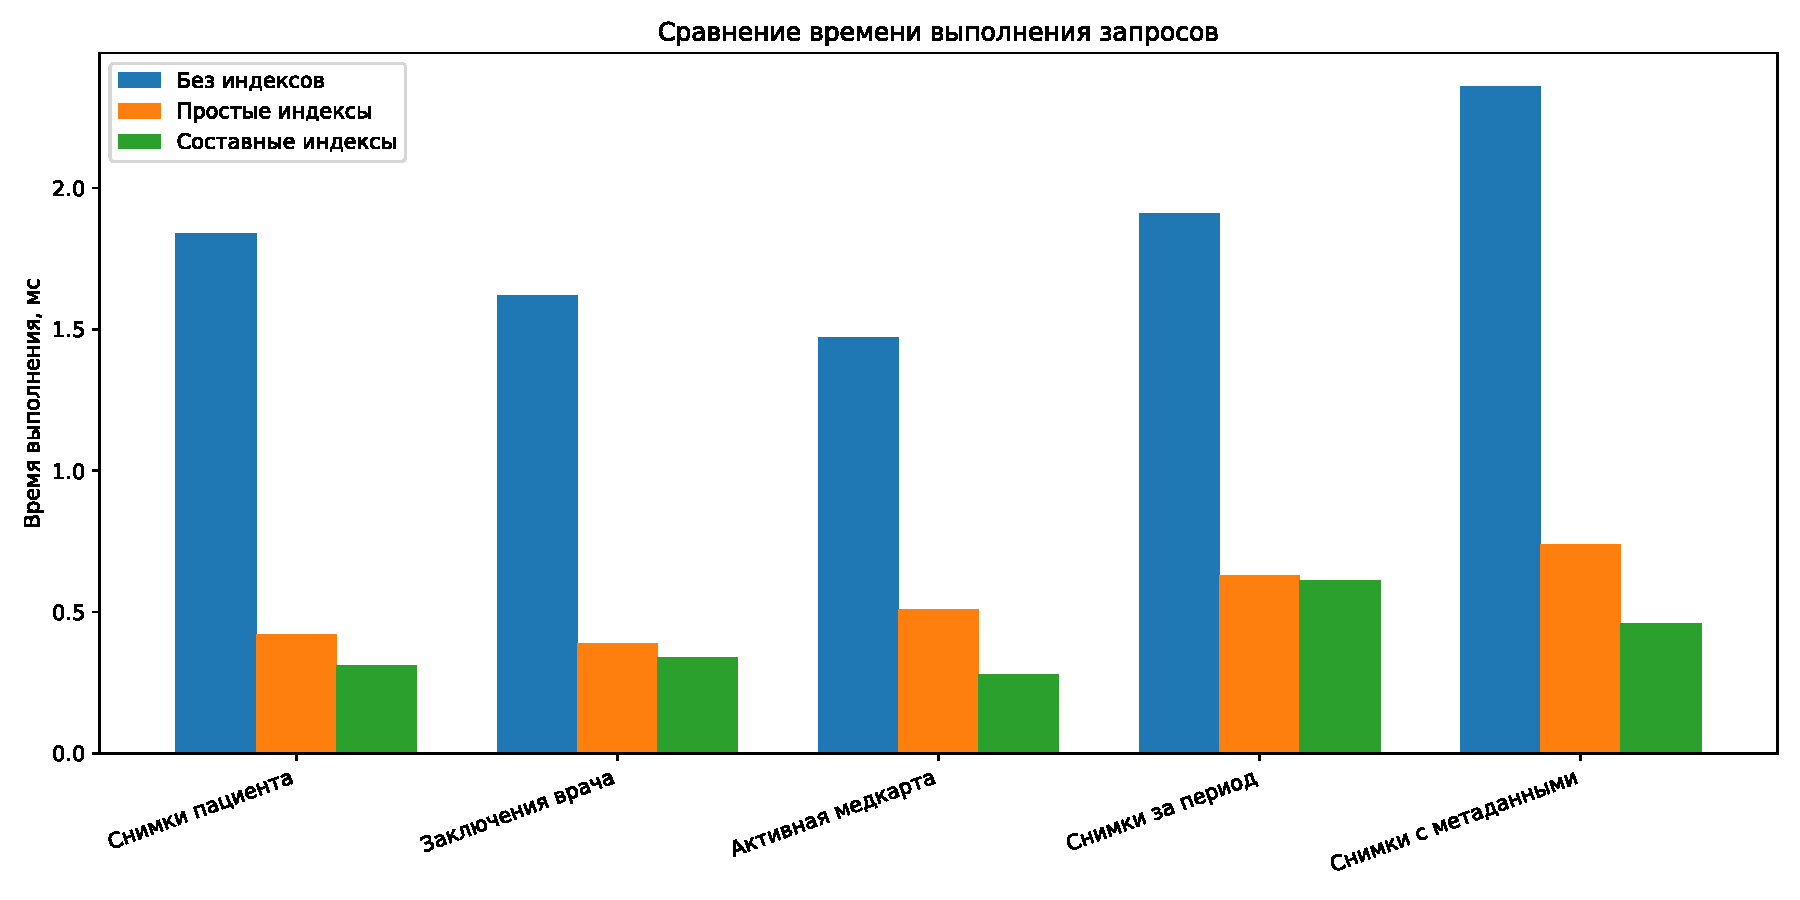
\includegraphics[width=\textwidth]{query_time_comparison}
	\caption{Сравнение времени выполнения запросов}
	\label{fig:query-time-comparison}
\end{figure}

По результатам видно, что использование индексов уменьшает время выполнения всех рассмотренных запросов. Наиболее заметное ускорение наблюдается для запросов, в которых фильтрация выполняется по внешним ключам, например по полям \texttt{patient\_id} и \texttt{doctor\_id}.

Для запроса получения активной медицинской карты пациента составной индекс \texttt{(patient\_id, is\_active)} оказался эффективнее набора простых индексов, так как оба поля одновременно используются в условии \texttt{WHERE}. Для запроса получения снимков пациента с метаданными составной индекс \texttt{(patient\_id, upload\_date)} также дал лучший результат, так как запрос сочетает фильтрацию по пациенту и сортировку по дате загрузки.

\section{Оценка ускорения запросов}

Для оценки эффективности индексирования было рассчитано ускорение выполнения запросов. Ускорение определялось по формуле:

\begin{equation}
	S = \frac{T_{\text{без индексов}}}{T_{\text{с индексом}}},
\end{equation}

где $T_{\text{без индексов}}$ --- время выполнения запроса без дополнительных индексов, $T_{\text{с индексом}}$ --- время выполнения запроса после создания индекса.

Результаты расчёта ускорения представлены в таблице~\ref{tbl:index-speedup}.

\begin{table}[H]
	\centering
	\caption{Ускорение выполнения запросов}
	\label{tbl:index-speedup}
	\small
	\resizebox{\textwidth}{!}{
		\begin{tabular}{|c|p{7.5cm}|c|c|}
			\hline
			\textbf{№} & \textbf{Запрос} & \textbf{Ускорение с простыми индексами} & \textbf{Ускорение с составными индексами} \\
			\hline
			1 & Получение снимков пациента & 4.38 & 5.94 \\
			\hline
			2 & Получение заключений врача & 4.15 & 4.76 \\
			\hline
			3 & Получение активной медицинской карты пациента & 2.88 & 5.25 \\
			\hline
			4 & Получение снимков за период & 3.03 & 3.13 \\
			\hline
			5 & Получение снимков пациента с метаданными & 3.19 & 5.13 \\
			\hline
		\end{tabular}
	}
\end{table}

График ускорения запросов приведён на рисунке~\ref{fig:query-speedup}.

\begin{figure}[H]
	\centering
	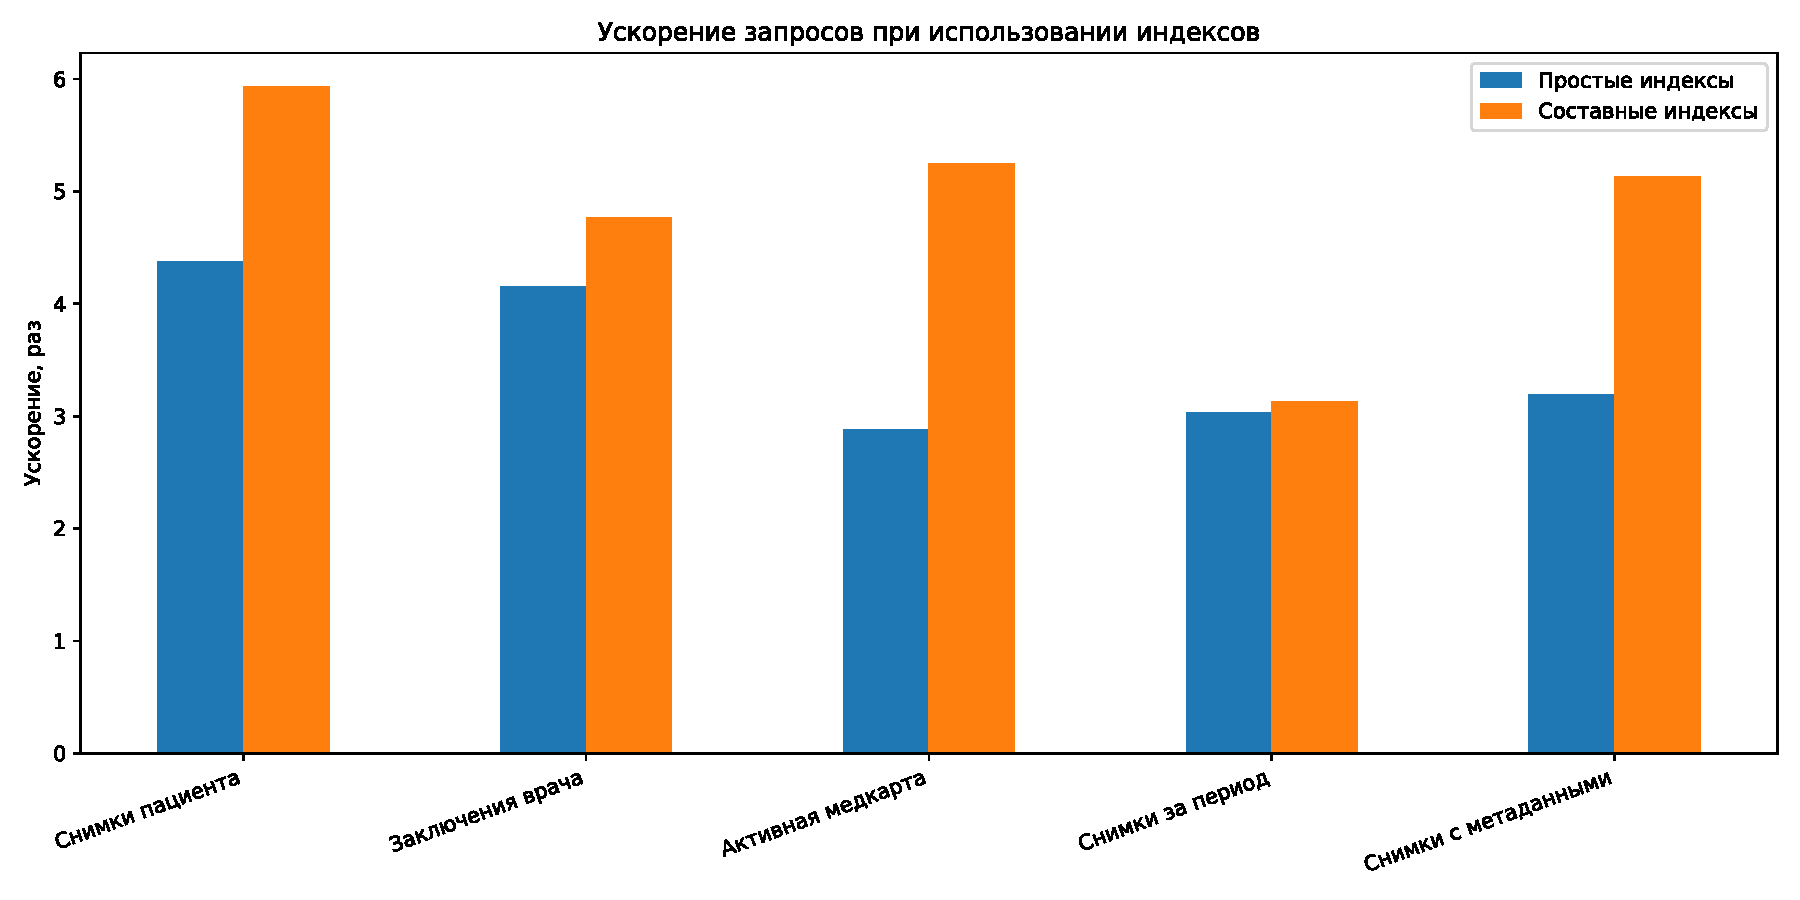
\includegraphics[width=\textwidth]{query_speedup}
	\caption{Ускорение запросов при использовании индексов}
	\label{fig:query-speedup}
\end{figure}

Среднее время выполнения запросов для трёх вариантов индексирования показано на рисунке~\ref{fig:average-query-time}.

\begin{figure}[H]
	\centering
	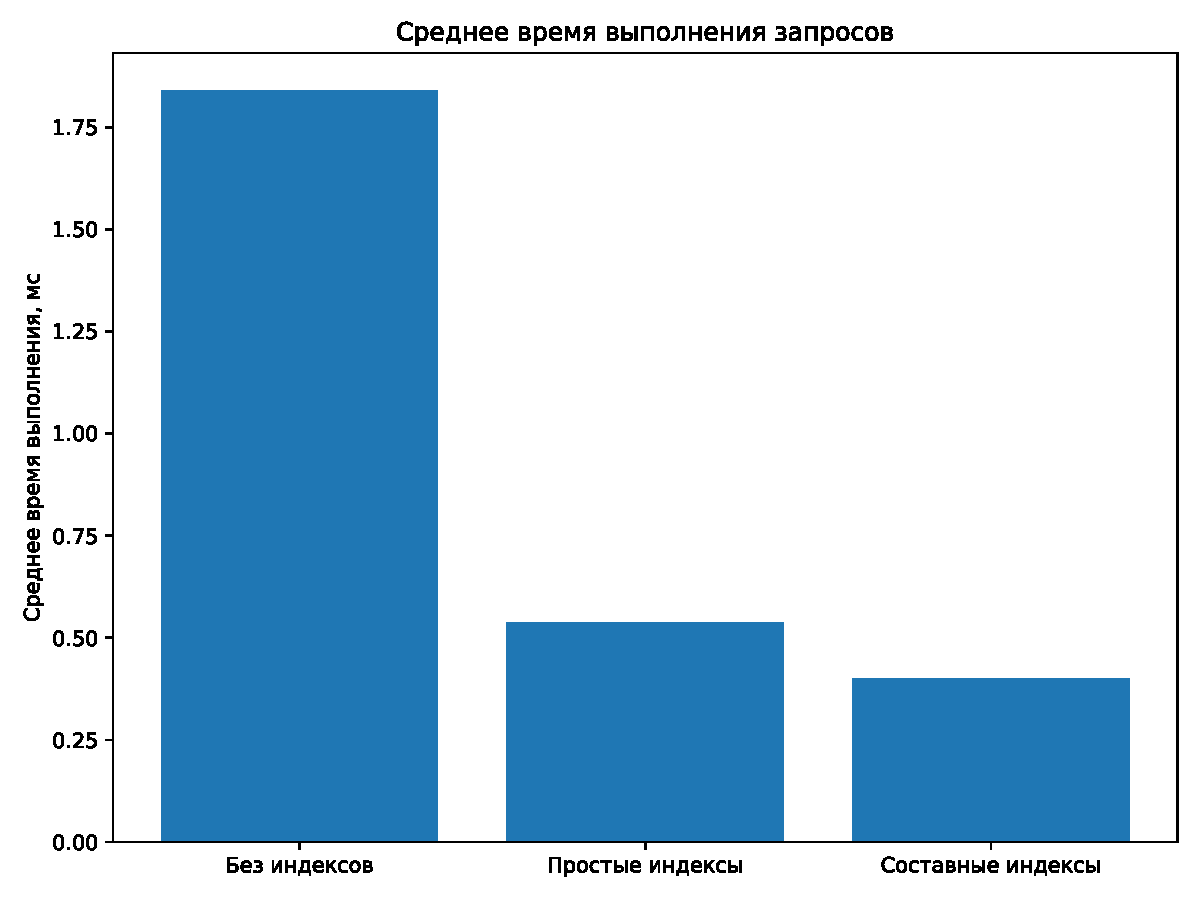
\includegraphics[width=0.75\textwidth]{average_query_time}
	\caption{Среднее время выполнения запросов}
	\label{fig:average-query-time}
\end{figure}

Среднее время выполнения запросов без дополнительных индексов составило 1.84 мс. После создания простых индексов среднее время уменьшилось до 0.54 мс. При использовании составных индексов среднее время выполнения составило 0.40 мс.

\section*{Вывод}

В результате исследования было установлено, что использование индексов оказывает положительное влияние на время выполнения типовых запросов к базе данных DentoBase.

Простые индексы позволяют ускорить запросы, выполняющие фильтрацию по одному полю. Составные индексы оказываются наиболее эффективными в тех случаях, когда запрос использует несколько условий фильтрации или сочетает фильтрацию и сортировку.

Наибольшее ускорение было получено для запроса получения снимков пациента и запроса получения активной медицинской карты. Это объясняется тем, что структура составных индексов соответствует структуре условий в запросах.

Таким образом, для разработанной базы данных целесообразно использовать индексы по внешним ключам, а также составные индексы для наиболее часто выполняемых запросов. Применение индексов позволило сократить время выполнения исследуемых запросов примерно в 3--6 раз.